\chapter{Detector commissioning}
\label{sec:commissioning}

By the end of $2019$, the commissioning of the SuperNEMO demonstrator has begun and first calorimeter data were taken.\\
To clarify, we give some common terms used in the detector assembly.
The calorimeter of SuperNEMO is segmented in $712$ optical modules (OM), each composed by the coupling of a photomultiplier tube (PMT) and a polystyrene scintillator (see sec.~\ref{sec:calorimeter} for more details).
The divider of a PMT is connected to $2$ cables, one providing the high voltage (HV), the other one, called signal cable, is a coaxial cable collecting and transporting the charge provided by the PMT.\\
By the summer $2020$, the SuperNEMO demonstrator will be encapsulated in an anti radon tent (\textcolor{red}{abbrev?}).
The so called \emph{patch panel} (PP) will insure passage of cables from inside, to outside the anti radon tent, doubling the amount of cables needed for the calorimeter.
We commonly talk about \emph{internal} cables (from detector to patch panel) and \emph{external} cables (from patch panel to electronics).
Consequently, regarding only the calorimeter part, 2848 cables were cut, assembled, connector-mounted, transported and installed at Modane.
Then checking cables condition is unavoidable to control and eventually fix the cables.

\section{Reflectometry tests}
\label{sec:reflecto}

\subsection{Principle and goal}

\emph{Reflectometry} tests were performed at Modane to check the condition of signal cables:
electronic pulses are generated at electronic boards and sent in each signal cable.
After propagation in the cable from electronics to calorimeter, the signal is reflected at PMT divider and propagate again in the cable from calorimeter to electronics.
Then the back pulse is recorded.
A thousand of pulses are sent in each cable, to test each PMT.
Analysing the shape and arrival time of those back pulses will allow us to check the signal cable conditions and control their length.
Controlling the length of cable is important
\begin{itemize}
\item to control if no inversions were made during calorimeter cabling: all external signal cables are $7$ meters-long (the distance between electronics and patch panel being the same for all channels), but internal cables length have been adapted to fit the distance from the patch panel to each optical module;
\item to check if each cable were cut at the right length;
\item to estimate the delay of signal due to cable lengths: the velocity of electrons in cables has a regular value that delays the signal comming from the PMT. This time delay depends on the cable length and has to be characterised for each cable.
\end{itemize}

Taking into account the final demonstrator design, each cable length were determined, coaxial cables were cut and labelled in LAL, Orsay.
To check if the cables were cut at right lengths and if no inversions were made at Modane when connecting cables, we check each cable length.
To do so, we send at electronics a pulse, called \emph{primary} pulse, in a given cable.
The signal will travel from electronics to the PMT through the cable.
As the PMT is not alimented (the HV is turned off during this data taking), the impedance at PMT is infinite, and the signal reflects at PMT divider.
Then the signal travels back from the PMT to the electronics, were it will be recorded by the acquisition.
This recorded back pulse is called \emph{secondary} pulse.


\subsection{Data taking at LSM}
\textcolor{red}{Explain the pulse sending principle with Jihane's documentation}
\subsection{Analysis}

\subsection*{Pulse timing: checking cable lengths}
\label{subsec:timing}

We determine the difference between the time of primary pulse and the time of secondary pulse.
Knowing the velocity of electrons in coaxial cables, we can deduce the corresponding cable length.
This measure is repeated for each PMT, allowing us to characterise all coaxial cables.\\
The propagation velocity of electrons in coaxial cables $v_{p}$ is a parameter, given as a percentage of the light speed in vaccuum c, as
\begin{equation*}
  v_{p}=\frac{1}{\sqrt{\epsilon}}\,\text{,}
\end{equation*}
with $\epsilon$ the dielectric constant of the material.
For the coaxial cables chosen for the demonstrator, this velocity is $69\%$.

We define the time of a pulse with a Constant Fraction Discriminator (CFD) parameterised by the fraction f, as represented in fig.~\ref{fig:CFD}.
We studied the influence of this fraction on the time measurement precision (see Sec.~\ref{subsec:CFD}).
In the following, we use $\text{f} = 40\%$.
The cable length $\mathcal{L}$ is therefore defined as $\mathcal{L}= 0.5\,\mathcal{T}\,v_{p}$, with $\mathcal{T}$ the round trip time from electronics to PMT divider, defined as
\begin{equation}
\mathcal{T} = \braket{\text{t}_{\text{secondary pulse}}-\text{t}_{\text{primary pulse}}}_{\text{p}} \, \text{,}
\end{equation}
 $\braket{}_{\text{p}}$ being the average over all pulses sent in one cable, and $\text{t}_{\text{i}}$ the time of pulse i.
For one signal cable, the mean signal timing (over all pulses sent in this cable) is calculated.
We repeat this operation for all signal cables.

A study was also performed to experimentally check the given signal celerity in cables (see Sec.~\ref{subsec:velocity}).


\subsection*{Checking the pulse amplitude attenuation}
When the signal travels in a cable, its amplitude is attenuated.
Then, another test for controlling the cable condition is to check if this attenuation matches the expectations (i.e. the value given by constructor).
We define the amplitude of a pulse as the maximum of this pulse, compared to the baseline.
The attenuation $\mathcal{A}$ of a given cable is then defined as $\mathcal{A}=\braket{\text{A}_{ \text{secondary pulse}}-\text{A}_{ \text{primary pulse}}}_{\text{p}}$, $\text{A}_{\text{i}}$ the amplitude of the pulse i.
A map summarising the attenuation for each cable is presented.

\subsection*{Checking the constructor signal velocity in cables}
\label{subsec:velocity}
As we want to check the celerity of signal given by Axon, we used $3$ cables of different lengths (see Fig.~\ref{fig:cable_lengths}).
Knowing the length of a cable, we determine the time needed for the signal to make a round trip in the cable, and conclude about the celerity of signal in each cable.
We found that the mean celerity on the $3$ cables is $0.7$ c, a bit greater than the celerity given by Axon of $0.69$ c.


\subsection*{Studying influence of CFD on the signal timing study}
\label{subsec:CFD}

\subsection*{Correction on event times}
\label{subsec:time_correction}

The main goal of this study was to check the lengths of signal cables.
We can also use the results to correct the time of recorded events.
Given that what we later define as an \emph{event} is firstly an electric signal, we should take into account the time for the signal to travel through cables.
This become possible with the reflectometry study we performed.
Knowing real lengths of cables and using the celerity of the signal, we deduce the time needed for the signal to travel from one given PMT divider to the electronics.
Then we can correct event times.

\subsection*{Pulse shape analysis}
\label{subsec:pulse_shape}


\subsection{Results}



\section{Calibrating the electronics}
\label{sec:TimeSynchroFEB}

\subsection{Principle}
\subsection{Measuring the time offset of front end boards}
\subsection{Results}

\begin{figure}
  \centering
  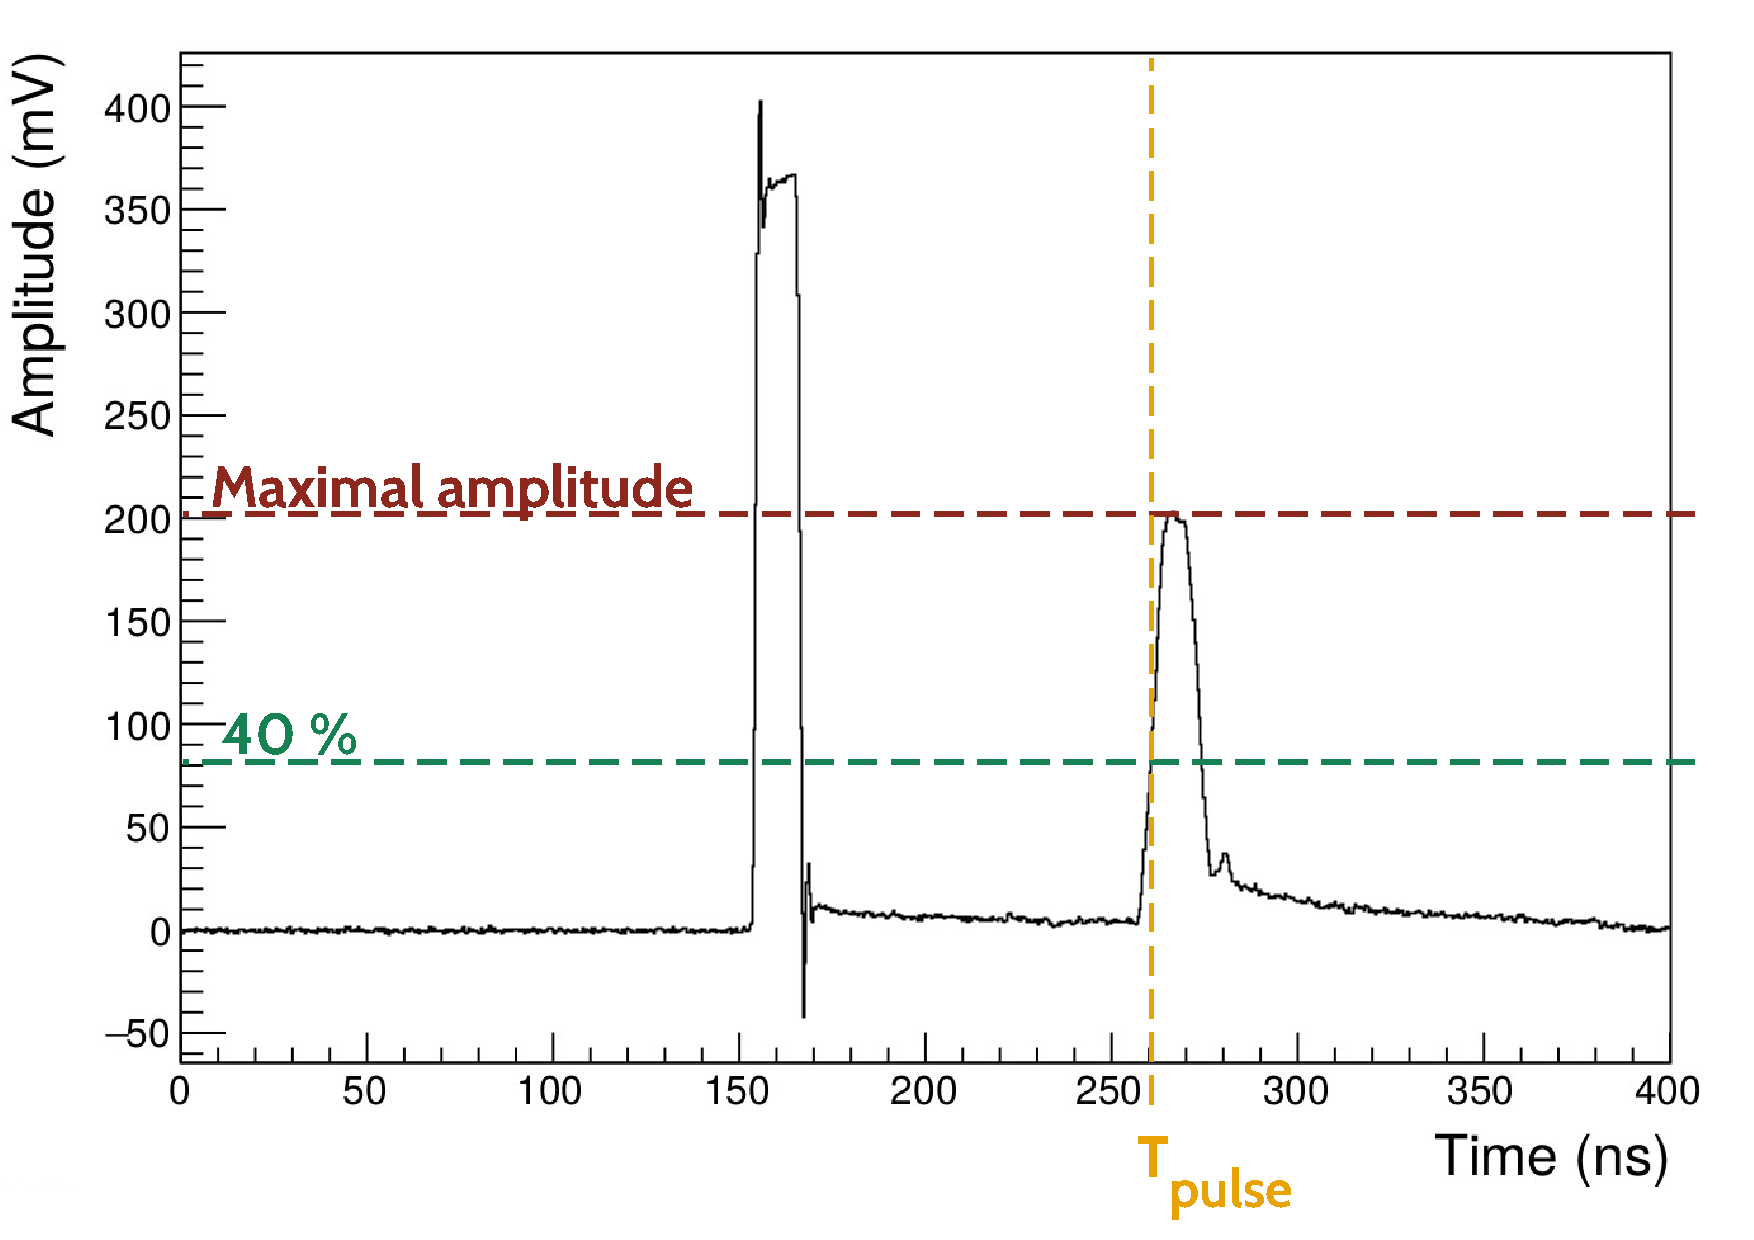
\includegraphics[width=10cm]{commissioning/fig_commissioning/CFD_example.pdf}
  \label{fig:CFD}
  \caption{In black is an example of a waveform with primary pulse (left) and secondary pulse (right).
    A representation of time CFD is given for the secondary pulse.
    Its maximal amplitude (red dotted line) and its fraction for $\text{f}=40\%$ (green dotted line) are displayed.
    The time $\text{T}_{\text{pulse}}$ (orange dotted line) reprensents the time of the secondary pulse calculated with a CFD at $\text{f}=40\%$.}
\end{figure}

\begin{figure}
  \centering
  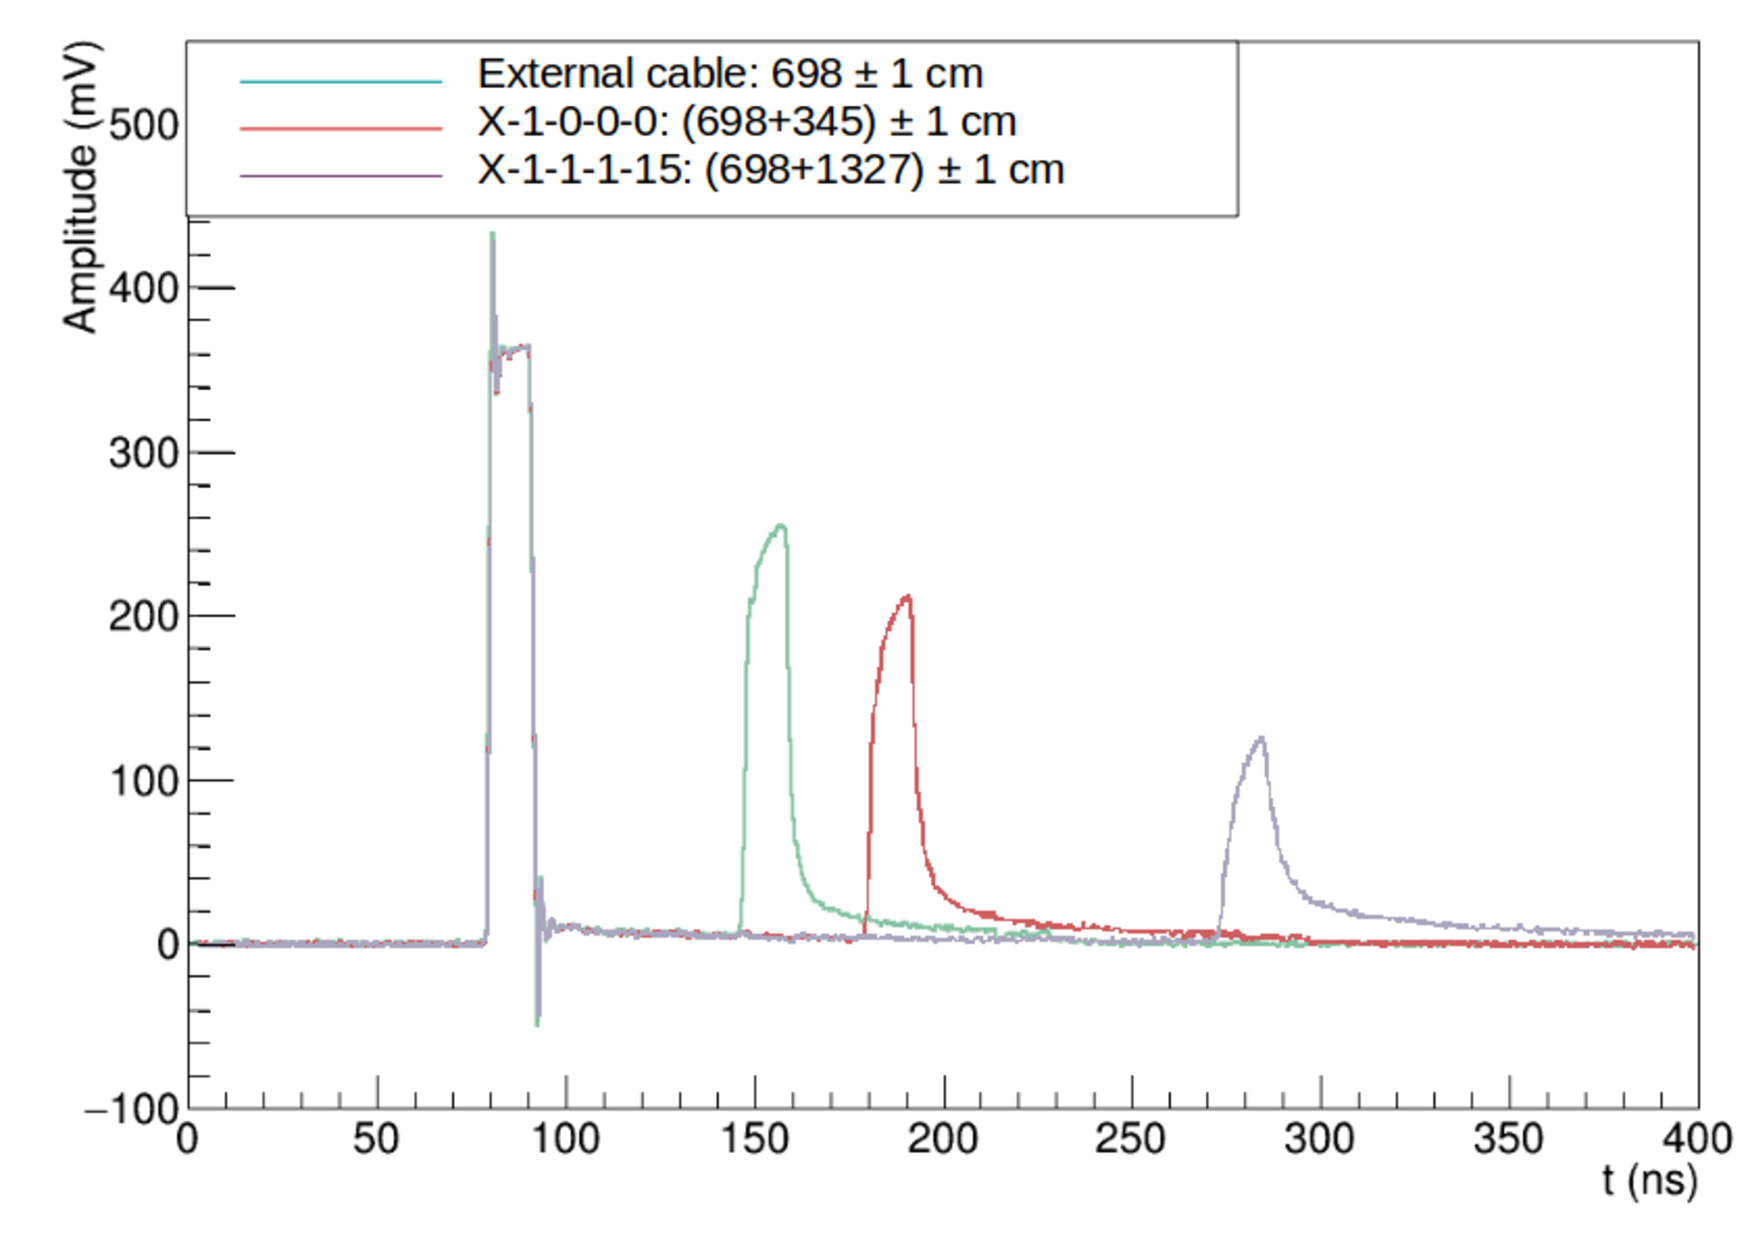
\includegraphics[width=10cm]{commissioning/fig_commissioning/length_tests.pdf}
  \label{fig:cable_lengths}
  \caption{Primary and secondary pulses for a $698 \pm 1$ cm cable (green), a $1043 \pm 1$ cm cable (red) and a $2025 \pm 1$ cm cable (grey).}
\end{figure}
